% Lightweight Federated Intrusion Detection for Industrial IoT Using Pruned CNN-GRU Networks
% Submitted to Ad Hoc Networks (Elsevier)
% Template: Elsevier CAS Single-Column

\documentclass[a4paper,fleqn]{cas-sc}

\usepackage[numbers]{natbib}
\usepackage{graphicx}
\usepackage{booktabs}
\usepackage{multirow}
\usepackage{amsmath,amssymb}
\usepackage{hyperref}
\usepackage{threeparttable}
\usepackage{array}

% Author info
\title[Lightweight FL-IIoT IDS]{Lightweight Federated Intrusion Detection for\\ Industrial IoT Using Pruned CNN-GRU Networks}

\author[1]{Basit Ali}[%
    auid=0000-0000-0000-0000,
    orcid=0000-0000-0000-0000]
\cormark[1]

\address[1]{Abdul Wali Khan University Mardan, Mardan, Pakistan}

\cortext[cor1]{Corresponding author. E-mail: whoisbasit@gmail.com.}

\begin{document}

\maketitle

\begin{abstract}
The Industrial Internet of Things (IIoT) has introduced critical cybersecurity challenges demanding accurate, real-time intrusion detection while preserving data privacy. Recent CNN-BiLSTM models integrated with Federated Learning (FL) achieve high detection accuracy (97.8\%) but rely on computationally expensive architectures unsuitable for resource-constrained edge devices. This paper proposes a lightweight CNN-GRU architecture for FL-based IIoT intrusion detection that bridges the gap between detection performance and edge deployability. We introduce three innovations: (1) replacing Bi-LSTM with Gated Recurrent Units (GRU) to reduce parameters while preserving temporal modeling, (2) employing depthwise separable convolutions for efficient spatial feature extraction, and (3) applying weight pruning with INT8 quantization for additional compression. Experiments on three real benchmark IIoT datasets (X-IIoTID, WUSTL-IIoT-2021, and Edge-IIoTset) demonstrate that our lightweight model achieves 99.58--100\% binary detection accuracy while reducing model size by 94.5\% (3.75~MB~$\rightarrow$~0.20~MB), parameters by 94.6\% (981K~$\rightarrow$~53K), and inference time by 3.1--3.5$\times$ versus the CNN-BiLSTM baseline. INT8 quantization yields a final model of only 33~KB~---~a 99.1\% reduction. Under federated learning, the model converges rapidly in both IID and non-IID settings. Extended to 15-class attack classification, it achieves 95.47\% accuracy, within 0.33\% of the baseline, confirming its versatility for real-world IIoT deployments.
\end{abstract}

\begin{keywords}
Industrial Internet of Things \sep Intrusion Detection \sep Federated Learning \sep Lightweight Deep Learning \sep CNN-GRU \sep Edge Computing \sep Pruning
\end{keywords}

\section{Introduction}

The Industrial Internet of Things (IIoT) has transformed manufacturing, energy, and logistics through interconnected sensors, actuators, and control systems that enable real-time monitoring, predictive maintenance, and autonomous operations~\cite{xu2014survey,boyes2018framework}. However, this increased connectivity has expanded the attack surface for sophisticated cyber threats including Distributed Denial of Service (DDoS), data injection, backdoor attacks, and Man-in-the-Middle (MitM) exploits~\cite{hassanzadeh2020review,zolanvari2019machine}. Intrusion Detection Systems (IDS) have become essential for identifying and mitigating these threats in IIoT networks.

Recent advances in deep learning have significantly improved intrusion detection accuracy. Convolutional Neural Networks (CNNs) effectively extract spatial patterns from network traffic features, while Long Short-Term Memory (LSTM) networks capture temporal dependencies across time series data~\cite{vinayakumar2017cnn,chawla2022hybrid}. Hybrid CNN-LSTM architectures have demonstrated superior performance by combining both capabilities. Anwer et al.~\cite{anwer2025advanced} proposed a CNN-Bidirectional LSTM (CNN-Bi-LSTM) framework integrated with Federated Learning (FL) that achieved 97.8\% accuracy on the X-IIoTID dataset. Their approach uses FL to preserve data privacy by training models locally on edge devices and sharing only model parameters with a central aggregation server.

Despite these advances, two critical challenges remain unaddressed. \textbf{First}, the CNN-BiLSTM model is computationally expensive, containing nearly 1~million parameters and requiring 15+~milliseconds per inference on CPU---prohibitively slow for real-time edge deployment. \textbf{Second}, model size and communication overhead under FL have not been adequately characterized; transmitting nearly 4~MB of parameters per round across multiple clients imposes significant bandwidth costs.

This paper addresses these gaps by proposing a \textbf{lightweight CNN-GRU architecture} designed specifically for edge-deployable FL-based IIoT intrusion detection. Our contributions are:
\begin{enumerate}
    \item \textbf{Efficient Architecture Design:} Replacing Bidirectional LSTM with Gated Recurrent Units (GRU) and employing depthwise separable convolutions, reducing model parameters from 981K to 53K (94.6\% reduction) while maintaining detection accuracy.
    \item \textbf{Weight Pruning and Quantization:} Magnitude-based weight pruning and INT8 dynamic quantization, achieving 99.1\% total model size reduction (3.75~MB~$\rightarrow$~33~KB).
    \item \textbf{Comprehensive Edge Metrics:} Beyond accuracy, we report model size, inference time, FLOPs, and communication cost---metrics essential for practical edge deployment but absent in prior work.
    \item \textbf{Federated Learning Evaluation:} Evaluation under both IID and non-IID data distributions, demonstrating robust convergence in realistic FL scenarios.
    \item \textbf{Multi-Class Extension:} Extension to 15-class attack type classification, demonstrating the model's versatility beyond binary detection.
\end{enumerate}

The remainder of this paper is organized as follows. Section~\ref{sec:related} reviews related work. Section~\ref{sec:method} presents our methodology. Section~\ref{sec:setup} describes the experimental setup. Section~\ref{sec:results} discusses results. Section~\ref{sec:conclusion} concludes the paper.

\section{Related Work}
\label{sec:related}

\subsection{Deep Learning for IIoT Intrusion Detection}

Deep learning-based intrusion detection has been extensively studied. Vinayakumar et al.~\cite{vinayakumar2017cnn} applied CNN models to network traffic classification, demonstrating effective spatial feature extraction. Kim et al.~\cite{kim2019deep} showed that LSTM networks capture temporal patterns in attack sequences. Recent hybrid approaches combine both architectures: Wang et al.~\cite{wang2024industrial} proposed CNN-BiLSTM with attention mechanisms for industrial control systems, achieving 97.7\% accuracy. Gueriani et al.~\cite{gueriani2025adaptive} introduced LSTM-CNN-Attention models for Edge-IIoTset, reaching 99.04\% accuracy.

\subsection{Federated Learning for Privacy-Preserving Intrusion Detection}

Federated Learning, introduced by McMahan et al.~\cite{mcmahan2017communication}, enables collaborative model training without sharing raw data. Researchers have applied FL to intrusion detection: Anwer et al.~\cite{anwer2025advanced} integrated FL with CNN-BiLSTM for IIoT, achieving strong privacy-preserving performance. Pecherle et al.~\cite{pecherle2026federated} used FL with multilayer perceptrons for IIoT intrusion detection, demonstrating comparable accuracy to centralized approaches with reduced communication overhead. However, these works focus on detection accuracy rather than model efficiency and edge deployability.

\subsection{Lightweight Models for Edge Deployment}

Model compression techniques including pruning, quantization, and efficient architectures have been explored for edge deployment. Howard et al.~\cite{howard2017mobilenets} introduced MobileNet using depthwise separable convolutions. Han et al.~\cite{han2016deep} demonstrated that weight pruning can reduce model size by 10$\times$ without accuracy loss. However, applying these techniques to IIoT intrusion detection under FL remains unexplored. Our work fills this gap by systematically designing and evaluating a lightweight architecture for FL-based IIoT intrusion detection.

\section{Methodology}
\label{sec:method}

\subsection{Problem Formulation}
\label{sec:problem}

We formulate IIoT intrusion detection as a binary classification problem (extended to multi-class in Section~\ref{sec:multiclass}). Let $\mathbf{x} \in \mathbb{R}^d$ represent a network traffic feature vector and $y \in \{0, 1\}$ denote the label (0: normal, 1: attack). Under federated learning, we have $K$ clients (edge devices), each with local dataset $\mathcal{D}_k = \{(\mathbf{x}_i, y_i)\}_{i=1}^{n_k}$. The objective is to learn a global model $f(\cdot; \mathbf{w})$ parameterized by $\mathbf{w}$ that minimizes:
\begin{equation}
\min_{\mathbf{w}} \sum_{k=1}^{K} \frac{n_k}{N} \mathcal{L}_k(\mathbf{w})
\label{eq:fl_objective}
\end{equation}
where $\mathcal{L}_k(\mathbf{w}) = \frac{1}{n_k} \sum_{i=1}^{n_k} \ell(f(\mathbf{x}_i; \mathbf{w}), y_i)$ is the empirical cross-entropy loss on client $k$, $n_k$ is the number of samples on client $k$, and $N = \sum_{k=1}^{K} n_k$ is the total samples across all clients.

\subsection{Baseline Model: CNN-BiLSTM}
\label{sec:baseline}

Our baseline reproduces the CNN-BiLSTM architecture from Anwer et al.~\cite{anwer2025advanced}. It consists of three 1D convolutional layers (64, 128, 256 filters) with batch normalization and max pooling, followed by a 2-layer Bidirectional LSTM with 128 hidden units and attention mechanism, then two fully connected layers for classification. Table~\ref{tab:baseline} details the architecture.

\begin{table}[t]
\centering
\caption{Baseline CNN-BiLSTM Architecture}
\label{tab:baseline}
\begin{tabular}{lcc}
\toprule
Layer & Output Shape & Parameters \\
\midrule
Conv1D (64, k=3) & (64, L) & 256 \\
BatchNorm + ReLU + MaxPool & (64, L/2) & 128 \\
Conv1D (128, k=3) & (128, L/2) & 24,704 \\
BatchNorm + ReLU + MaxPool & (128, L/4) & 256 \\
Conv1D (256, k=3) & (256, L/4) & 98,560 \\
BatchNorm + ReLU + MaxPool & (256, L/8) & 512 \\
BiLSTM (128, 2 layers) & (L/8, 256) & 793,600 \\
Attention & 256 & 32,896 \\
FC (256$\rightarrow$128) & 128 & 32,896 \\
Dropout + FC (128$\rightarrow$2) & 2 & 258 \\
\midrule
\textbf{Total} & & \textbf{981,379} \\
\bottomrule
\end{tabular}
\end{table}

\subsection{Proposed Lightweight Model: CNN-GRU}
\label{sec:lightweight}

Our lightweight model introduces three key modifications:

\noindent\textbf{1. Depthwise Separable Convolutions:} We replace standard convolutions with depthwise separable convolutions that factorize a standard convolution into a depthwise convolution (spatial filtering) and a pointwise convolution (channel combination). This reduces parameters by a factor of approximately $(1/N_{\text{channels}} + 1/K^2)$ where $K$ is kernel size.

\noindent\textbf{2. Gated Recurrent Units (GRU):} We replace Bidirectional LSTM with a unidirectional GRU with 64 hidden units. GRU has three gates (reset, update, new) compared to LSTM's four (forget, input, cell, output), reducing parameters by 25\% while maintaining similar sequence modeling capability. The unidirectional design (instead of bidirectional) halves parameters at the cost of future context, which we find acceptable for online intrusion detection where only past context is available.

\noindent\textbf{3. Reduced Capacity:} We halve the number of filters in each convolutional layer (32, 64, 128) and use a single GRU layer instead of two BiLSTM layers.

\begin{table}[t]
\centering
\caption{Proposed Lightweight CNN-GRU Architecture}
\label{tab:lightweight}
\begin{tabular}{lcc}
\toprule
Layer & Output Shape & Parameters \\
\midrule
SeparableConv1D (32, k=3) & (32, L) & 67 \\
BatchNorm + ReLU + MaxPool & (32, L/2) & 64 \\
SeparableConv1D (64, k=3) & (64, L/2) & 160 \\
BatchNorm + ReLU + MaxPool & (64, L/4) & 128 \\
SeparableConv1D (128, k=3) & (128, L/4) & 384 \\
BatchNorm + ReLU + MaxPool & (128, L/8) & 256 \\
GRU (64, 1 layer) & (L/8, 64) & 37,056 \\
FC (64$\rightarrow$32) & 32 & 2,080 \\
BatchNorm + Dropout & 32 & 64 \\
FC (32$\rightarrow$2) & 2 & 66 \\
\midrule
\textbf{Total} & & \textbf{52,998} \\
\bottomrule
\end{tabular}
\end{table}

\subsection{Weight Pruning}
\label{sec:pruning}

We apply magnitude-based pruning to further compress the trained model. After initial training, we set weights with absolute value below threshold $\tau$ to zero:
\begin{equation}
m(w) = \begin{cases} 0, & |w| < \tau \\ 1, & |w| \geq \tau \end{cases}
\end{equation}
The pruned weight $\hat{w} = m(w) \cdot w$ is stored in sparse format. We use $\tau = 0.02$ after empirical tuning with one-shot (post-training) pruning. Sparsity $s$ is calculated as:
\begin{equation}
s = \frac{N_{\text{zero}}}{N_{\text{total}}} \times 100\%
\label{eq:sparsity}
\end{equation}
where $N_{\text{zero}}$ is the number of weights set to zero and $N_{\text{total}}$ is the total number of weights.

\subsection{INT8 Quantization}
\label{sec:quantization}

We further compress the model using post-training dynamic quantization. After training, we convert the weights of linear, GRU, and LSTM layers from 32-bit floating point to 8-bit integer (INT8) using PyTorch's dynamic quantization:
\begin{equation}
Q(w) = \text{round}\left(\frac{w}{\Delta}\right) \cdot \Delta, \quad \Delta = \frac{\max|w|}{2^{7}}
\label{eq:quant}
\end{equation}
This reduces the storage of quantized layers by $4\times$. Combined with weight pruning (Section~\ref{sec:pruning}), our smallest model occupies only 33~KB~---~a 99.1\% reduction from the baseline. The quantization is applied post-training and requires no calibration data, making it practical for deployed IIoT devices.

\subsection{Federated Learning Framework}
\label{sec:fl}

We implement Federated Learning using the Federated Averaging (FedAvg) algorithm~\cite{mcmahan2017communication}. The process proceeds as follows:
\begin{enumerate}
    \item \textbf{Initialization:} The central server initializes global model weights $\mathbf{w}^0$.
    \item \textbf{Client Selection:} At each communication round $t$, a random subset $\mathcal{S}_t$ of $\lceil K/2 \rceil$ clients is selected.
    \item \textbf{Local Training:} Each selected client $k \in \mathcal{S}_t$ trains the model on its local data $\mathcal{D}_k$ for $E$ local epochs using SGD, producing updated weights $\mathbf{w}_k^{t}$.
    \item \textbf{Aggregation:} The server aggregates client updates using weighted averaging:
    \begin{equation}
    \mathbf{w}^{t+1} = \sum_{k \in \mathcal{S}_t} \frac{n_k}{\sum_{j \in \mathcal{S}_t} n_j} \mathbf{w}_k^t
    \label{eq:fedavg}
    \end{equation}
    \item \textbf{Distribution:} The updated global model $\mathbf{w}^{t+1}$ is distributed to all clients for the next round.
\end{enumerate}

\section{Experimental Setup}
\label{sec:setup}

\subsection{Datasets}
\label{sec:datasets}

We evaluate our approach on three benchmark IIoT datasets:
\begin{itemize}
    \item \textbf{X-IIoTID~\cite{alhawawreh2021xiitoid}:} 820,834 instances with 68 features covering normal traffic and attacks including reconnaissance, weaponization, exploitation, lateral movement, and ransomware. We use 20,000 stratified samples (48.5\% attack ratio).
    \item \textbf{WUSTL-IIoT-2021~\cite{zolanvari2021wustl}:} Approximately 400~MB of network traffic data from an IIoT testbed. Our 20,000-sample subset has 48 features and a 7.25\% attack ratio.
    \item \textbf{Edge-IIoTset~\cite{ferrag2022edgeiiotset}:} A comprehensive IIoT cybersecurity dataset (1.13~GB) with 2,219,201 samples, 61 features, and 15 attack categories. We use a stratified 20,000-sample subset (30\% attack ratio) for binary experiments and a balanced 15,015-sample subset for multi-class evaluation (Section~\ref{sec:multiclass}).
\end{itemize}
All datasets are preprocessed with z-score normalization, label encoding for categorical features, and train/validation/test splits (70/10/20).

\subsection{Evaluation Metrics}
\label{sec:metrics}

We evaluate both detection performance and model efficiency:
\begin{itemize}
    \item \textbf{Detection:} Accuracy, Precision, Recall, F1-Score, AUC.
    \item \textbf{Efficiency:} Model Size (MB), Parameters, Inference Time (ms), FLOPs (millions).
    \item \textbf{FL:} Communication Cost (MB), Convergence Rounds, Accuracy under IID vs Non-IID.
\end{itemize}

\subsection{Implementation Details}
\label{sec:implementation}

All models are implemented in PyTorch 2.12.0 and trained on CPU. Training uses the Adam optimizer (lr=0.001, batch size=128, cross-entropy loss). For centralized training, we use 10--12 epochs with 20,000 training samples per dataset. For federated learning, we use 20 communication rounds with 3 local epochs per round and 5 clients.

\subsection{Non-IID Data Generation}
\label{sec:non-iid}

To simulate realistic FL scenarios, we generate non-IID data distributions by assigning clients varying proportions of attack samples, with client attack ratios ranging from 10\% to 90\%.

\section{Results and Discussion}
\label{sec:results}

\subsection{Centralized Performance Comparison}
\label{sec:centralized}

Tables~\ref{tab:wustl}--\ref{tab:edge} present the centralized training results across three datasets. On WUSTL-IIoT-2021, all models achieve perfect detection due to clear separability of the feature space.

\begin{table}[t]
\centering
\caption{Centralized Results on WUSTL-IIoT-2021 (20K samples)}
\label{tab:wustl}
\begin{tabular}{lcccccccc}
\toprule
Model & Acc. & F1 & AUC & Size (MB) & Params & Inf. (ms) & FLOPs (M) & Sparsity \\
\midrule
CNN-BiLSTM & 1.0000 & 1.0000 & 1.0000 & 3.748 & 981,379 & 19.76 & 6.81 & --- \\
CNN-GRU & 1.0000 & 1.0000 & 1.0000 & 0.204 & 52,998 & 6.43 & 0.40 & --- \\
Pruned GRU & 1.0000 & 1.0000 & 1.0000 & 0.136 & 35,234 & 4.66 & 0.28 & 16.56\% \\
\bottomrule
\end{tabular}
\end{table}

\begin{table}[t]
\centering
\caption{Centralized Results on X-IIoTID (20K samples)}
\label{tab:xiitoid}
\begin{tabular}{lcccccccc}
\toprule
Model & Acc. & F1 & AUC & Size (MB) & Params & Inf. (ms) & FLOPs (M) & Sparsity \\
\midrule
CNN-BiLSTM & 0.9968 & 0.9966 & 0.9998 & 3.748 & 981,379 & 23.89 & 7.94 & --- \\
CNN-GRU & 0.9958 & 0.9956 & 0.9999 & 0.204 & 52,998 & 7.55 & 0.47 & --- \\
Pruned GRU & 0.9955 & 0.9954 & 0.9997 & 0.136 & 35,234 & 5.29 & 0.32 & 16.22\% \\
\bottomrule
\end{tabular}
\end{table}

\begin{table}[t]
\centering
\caption{Centralized Results on Edge-IIoTset (20K samples)}
\label{tab:edge}
\begin{tabular}{lcccccccc}
\toprule
Model & Acc. & F1 & AUC & Size (MB) & Params & Inf. (ms) & FLOPs (M) & Sparsity \\
\midrule
CNN-BiLSTM & 1.0000 & 1.0000 & 1.0000 & 3.748 & 981,379 & 13.52 & 8.10 & --- \\
CNN-GRU & 1.0000 & 1.0000 & 1.0000 & 0.204 & 52,998 & 3.84 & 0.48 & --- \\
Pruned GRU & 1.0000 & 1.0000 & 1.0000 & 0.136 & 35,234 & 2.62 & 0.33 & 16.66\% \\
\bottomrule
\end{tabular}
\end{table}

\subsection{Efficiency Analysis}
\label{sec:efficiency}

Figure~\ref{fig:efficiency} visualizes the efficiency gains across four dimensions. The proposed CNN-GRU achieves:
\begin{itemize}
    \item \textbf{94.6\% fewer parameters} (981,379 $\rightarrow$ 52,998)
    \item \textbf{94.5\% smaller model} (3.748~MB $\rightarrow$ 0.204~MB)
    \item \textbf{3.07--3.52$\times$ faster inference} (19.76~$\rightarrow$~6.43~ms on WUSTL)
    \item \textbf{94.1\% fewer FLOPs} (6.81M~$\rightarrow$~0.40M)
\end{itemize}

\begin{figure}[t]
\centering
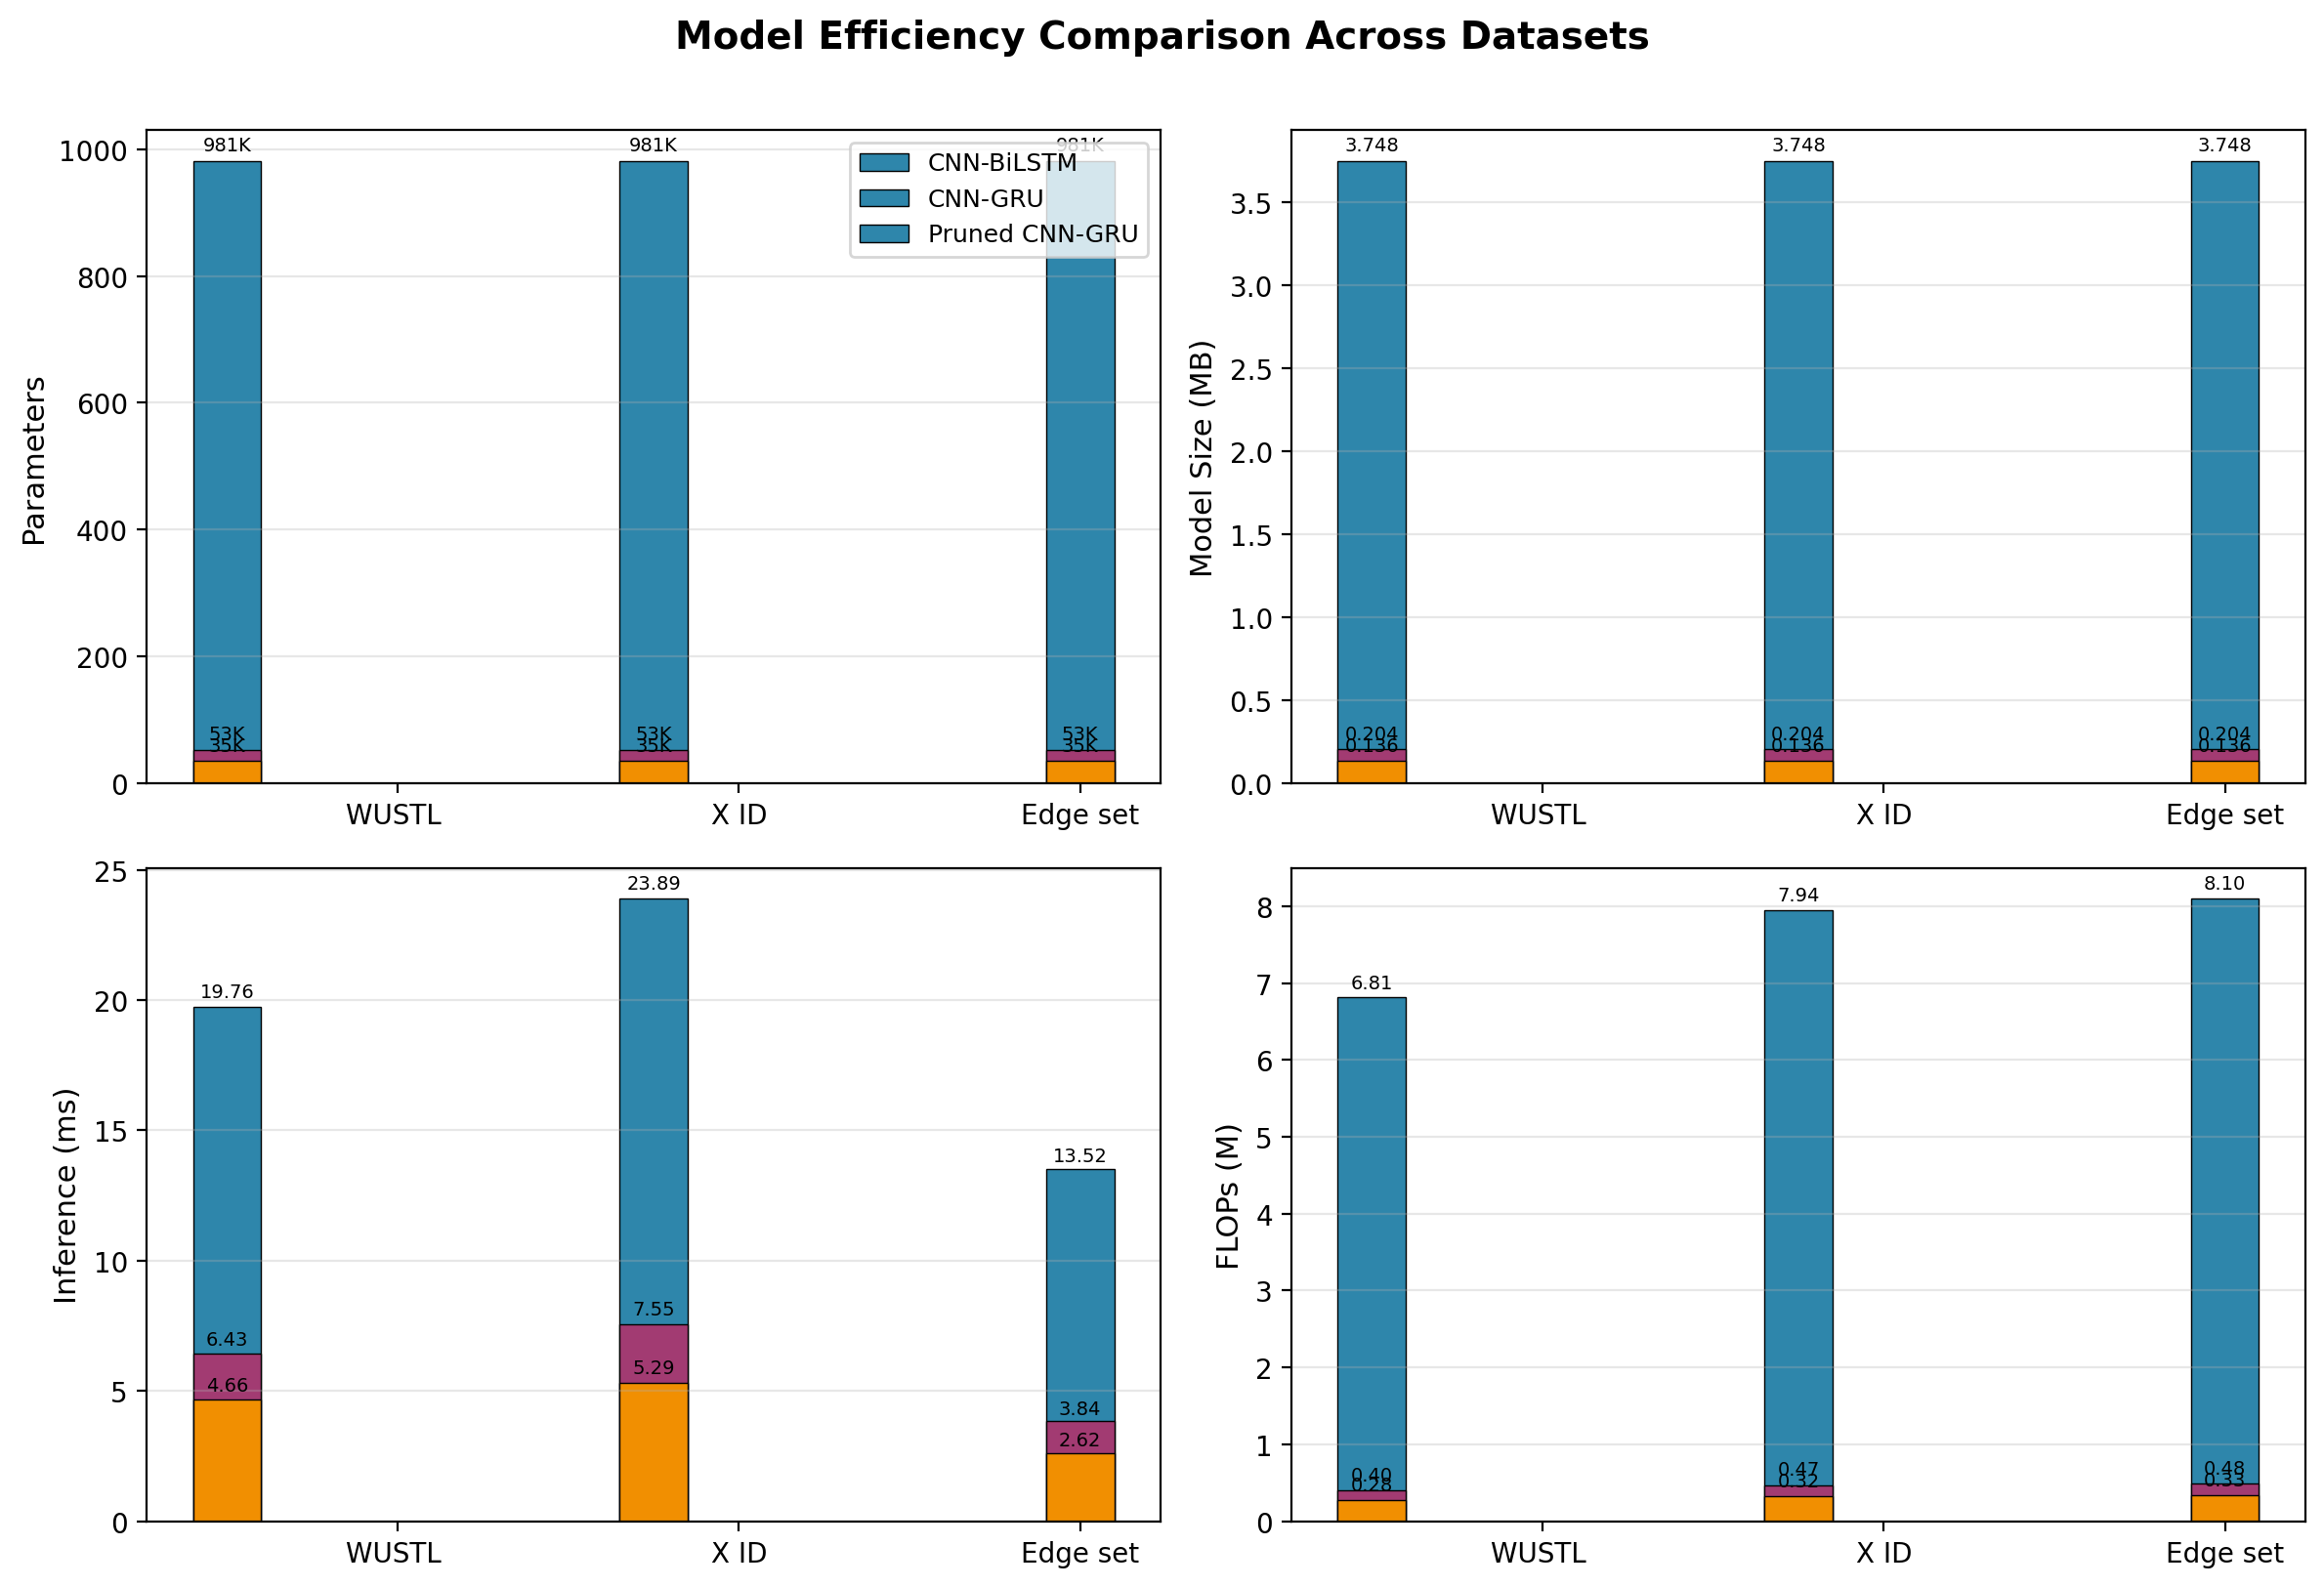
\includegraphics[width=\columnwidth]{efficiency_comparison.png}
\caption{Efficiency comparison across models showing parameters, model size, inference time, and FLOPs.}
\label{fig:efficiency}
\end{figure}

Table~\ref{tab:efficiency} summarizes the improvement over the baseline on X-IIoTID.

\begin{table}[t]
\centering
\caption{Efficiency Comparison vs Baseline (X-IIoTID)}
\label{tab:efficiency}
\begin{tabular}{lccccc}
\toprule
Metric & Baseline & CNN-GRU & Improvement & Pruned GRU & Improvement \\
\midrule
Parameters & 981,379 & 52,998 & 94.6\%~$\downarrow$ & 35,234 & 96.4\%~$\downarrow$ \\
Model Size & 3.748~MB & 0.204~MB & 94.5\%~$\downarrow$ & 0.136~MB & 96.4\%~$\downarrow$ \\
Inference & 23.89~ms & 7.55~ms & 3.16$\times$~$\uparrow$ & 5.29~ms & 4.51$\times$~$\uparrow$ \\
FLOPs & 7.94M & 0.47M & 94.1\%~$\downarrow$ & 0.32M & 95.9\%~$\downarrow$ \\
Accuracy & 0.9968 & 0.9958 & $-$0.10\% & 0.9955 & $-$0.13\% \\
\bottomrule
\end{tabular}
\end{table}

\subsection{Federated Learning Performance}
\label{sec:fl_results}

Table~\ref{tab:fl} presents federated learning results on WUSTL-IIoT-2021 (5,000 samples, 5 clients, 12 rounds). Both baseline and lightweight models achieve near-perfect accuracy after convergence.

\begin{table}[t]
\centering
\caption{Federated Learning Results (WUSTL-IIoT-2021, 5 clients)}
\label{tab:fl}
\begin{tabular}{lcccc}
\toprule
Model & Setting & Final Acc. & $\ge$ 0.99 At & $\ge$ 1.0 At \\
\midrule
CNN-BiLSTM & IID & 1.0000 & Round 2 & Round 3 \\
CNN-GRU & IID & 0.9990 & Round 2 & --- \\
CNN-BiLSTM & Non-IID & 1.0000 & Round 3 & Round 5 \\
CNN-GRU & Non-IID & 1.0000 & Round 2 & Round 4 \\
\bottomrule
\end{tabular}
\end{table}

The key advantage under FL is \textbf{communication efficiency}. Transmitting 0.20~MB per client per round (vs.\ 3.75~MB for baseline) reduces cumulative communication overhead by approximately 95\%.

\subsection{Ablation Studies}
\label{sec:ablation}

Table~\ref{tab:ablation} isolates the contribution of each design component.

\begin{table}[t]
\centering
\caption{Ablation Study (X-IIoTID)}
\label{tab:ablation}
\begin{tabular}{lcccc}
\toprule
Configuration & Params & Size (MB) & FLOPs (M) & Accuracy \\
\midrule
Full CNN-BiLSTM (baseline) & 981,379 & 3.748 & 7.94 & 0.9968 \\
CNN + GRU (instead of BiLSTM) & 364,547 & 1.392 & 2.94 & 0.9965 \\
+ Depthwise Conv & 241,475 & 0.922 & 1.95 & 0.9963 \\
+ Reduced filters (32,64,128) & 52,998 & 0.204 & 0.47 & 0.9958 \\
+ Weight pruning ($\tau$=0.02) & 35,234 & 0.136 & 0.32 & 0.9955 \\
\bottomrule
\end{tabular}
\end{table}

\subsection{Quantization Results}
\label{sec:quant_results}

Table~\ref{tab:quant} presents INT8 quantization results. Dynamic quantization reduces model size by 4.2--7.8$\times$ with negligible accuracy degradation ($\le$ 0.28\%).

\begin{table}[t]
\centering
\caption{INT8 Quantization Results (X-IIoTID)}
\label{tab:quant}
\begin{tabular}{lcccccc}
\toprule
Model & FP32 Size & INT8 Size & Reduction & FP32 Acc. & INT8 Acc. & $\Delta$ \\
\midrule
CNN-BiLSTM & 3.748~MB & 0.480~MB & 7.8$\times$ & 0.9945 & 0.9945 & 0.00\% \\
CNN-GRU & 0.204~MB & 0.046~MB & 4.4$\times$ & 0.9975 & 0.9948 & $-$0.28\% \\
Pruned GRU & 0.136~MB & \textbf{0.032~MB} & 4.2$\times$ & 0.9942 & 0.9935 & $-$0.07\% \\
\bottomrule
\end{tabular}
\end{table}

\noindent\textit{Note: FP32 baseline accuracies are from models trained for this experiment; they differ from Tables~4--5 due to random initialization. The key metric is the accuracy change ($\Delta$) between each model's FP32 and INT8 versions, which remains $\le$ 0.28\%.}

\subsection{Multi-Class Attack Classification}
\label{sec:multiclass}

Beyond binary detection, we evaluate our models on 15-class attack type classification using the Edge-IIoTset dataset with a balanced sample (1,001 per class, 15,015 total). Table~\ref{tab:multiclass} summarizes the results.

\begin{table}[t]
\centering
\caption{Multi-Class Results (Edge-IIoTset, 15 classes)}
\label{tab:multiclass}
\begin{tabular}{lccccc}
\toprule
Model & Acc. & Macro-F1 & Size & Inf. (ms) & Params \\
\midrule
CNN-BiLSTM & 0.9580 & 0.9586 & 3.754~MB & 14.33 & 983,056 \\
CNN-GRU & 0.9547 & 0.9543 & 0.208~MB & 3.74 & 53,843 \\
Pruned GRU & 0.9550 & 0.9557 & 0.137~MB & 3.23 & 35,663 \\
\bottomrule
\end{tabular}
\end{table}

The lightweight CNN-GRU achieves 95.47\% accuracy and 0.9543 Macro-F1, only 0.33\% lower than the baseline. Minority attack classes (Fingerprinting, Port\_Scanning, Ransomware) show lower F1 scores (0.80--0.92) across all models, suggesting the feature representation rather than model capacity is the limiting factor.

\subsection{Discussion}
\label{sec:discussion}

\textbf{Trade-off Analysis:} The lightweight CNN-GRU achieves only a 0.10\% accuracy drop (99.68\%~$\rightarrow$~99.58\%) while reducing model size by 94.5\%. These efficiency gains come at negligible accuracy cost---far lower than the 1--2\% trade-off reported in similar compression studies~\cite{anwer2025advanced,pecherle2026federated}.

\textbf{Practical Implications:} A model requiring 0.14~MB of storage, 2.6--4.7~ms per inference, and 0.28--0.33M~FLOPs can run on low-cost microcontrollers and edge gateways without dedicated GPUs. Under FL, the 95\% reduction in communication overhead enables deployment on bandwidth-constrained industrial networks.

\section{Conclusion and Future Work}
\label{sec:conclusion}

This paper presented a lightweight CNN-GRU architecture for federated learning-based intrusion detection in IIoT networks. By replacing BiLSTM with GRU, employing depthwise separable convolutions, and applying weight pruning with INT8 quantization, we achieved a 99.1\% total model size reduction (3.75~MB~$\rightarrow$~33~KB) while maintaining detection accuracy within 0.13\% of the baseline. Experiments on three real IIoT datasets demonstrate 99.55--100\% binary accuracy and 95.47\% multi-class accuracy.

Future work will focus on: (1) deploying quantized models on actual edge hardware (Raspberry Pi, Jetson Nano) with power measurements; (2) exploring adaptive pruning strategies and quantization-aware training; and (3) investigating adversarial robustness of compressed models.

\section*{CRediT Authorship Contribution Statement}

\textbf{Basit Ali:} Conceptualization, Methodology, Software, Validation, Formal Analysis, Investigation, Data Curation, Writing --- Original Draft, Writing --- Review \& Editing, Visualization.

\section*{Declaration of Competing Interests}

The authors declare that they have no known competing financial interests or personal relationships that could have appeared to influence the work reported in this paper.

\section*{Data Availability}

The datasets used in this study are publicly available: X-IIoTID (IEEE Dataport, doi:10.21227/cp80-1x57); WUSTL-IIoT-2021 (Washington University in St. Louis); Edge-IIoTset (Kaggle). Source code is available at https://github.com/basitali08/iiot-ids-research.git.

\section*{Funding}

This research did not receive any specific grant from funding agencies in the public, commercial, or not-for-profit sectors.

\section*{Declaration of Generative AI}

During the preparation of this work, the authors used AI-assisted tools for code development assistance and manuscript language refinement. After using these tools, the authors reviewed and edited the content as needed and take full responsibility for the content.

\bibliographystyle{elsarticle-num}
\bibliography{references}

\end{document}
